\section{Physics Analysis (Bertrand + Sophie + Andy)}
\label{sec:analysis}
%\textcolor{blue}{Scope: Describe existing analysis efforts methodologies.  Describe plans for a reference analysis.  Give an overview of techniques that we might apply, and an estimate of the scope of those in terms of data storage and processing needs.  Call out the use of AI/ML and possible use of hardware accelerators.}

Data analysis broadly refers to the ensemble of tools and techniques used to extract constraints on the physical properties of the muon. Data analysis tasks include for example measurements of muon branching fractions and capture rates, comparisons between data and Monte Carlo simulations, extraction of calibration and detector performance parameters, or search for new phenomena. For these tasks, the software framework used for large scale data processing might not be the most appropriate solution. This difference may not necessarily arise from missing functionalities or technological limitations in the large scale production framework, but might reflect the preference of analysts to trade capabilities in favor of flexibility and simplicity. The inclusion of external tools, such as machine learning or fit algorithms, might also be easier within a custom framework. Similarly, reduced data analysis samples (aka ntuples) might be more convenient to analyze that data records containing the full event information. These samples could be structured differently from the data recorded by the detector (e.g. columnar structure) to improve the processing performance. This section describes the analysis frameworks and reduced data samples used by the experiment, together with an application of these tools to a generic reference analysis.  


\subsection{Analysis Frameworks and Interfaces}
%\textcolor{red}{Sophie: we should discuss how the tuples/framework will support early data taking, and commissioing}

%To conduct offline analysis the output of the Mu2e reconstruction can be input into simplified ntuples. 
Offline analysis can be facilitated by the use of reduced data sets, both smaller in size and simpler in structure, generally consisting of a small set of C++ fundamental types (deemed the most useful for analyses) rather than Mu2e-specific data products. The smaller size reduces the need to prestage the files from tape and the simpler structure translates into a shallower learning curve for new users. The removal of the dependency on the full Mu2e software environment allows users to carry out analyses locally, which may carry some advantages. 


%\subsubsection{Existing Frameworks}

Mu2e currently has two ntuple frameworks: TrkAna and Stntuple. Both output ROOT-based structures. The data can be organized into event rows, allowing simple analysis macros to be written in either ROOT (C/C++) or python. Analysis groups have analysis frameworks running over the ntuples to generate plots and perform fits. When developing these tools we have been concerned with maintaining interfaces to both ROOT and python. A common python environment is used to facilitate interoperability between analysis groups. We already maintain a ROOT installation, Mu2e/Offline is always built against a specified ROOT release.



\subsubsection{TrkAna}

TrkAna provides a simple ROOT TTree structure. Each entry in the TTree corresponds to a single Mu2e event and contains reconstructed information extracted Mu2e data-products associated with the tracker, calorimeter, and CRV. There is also the option to write out Monte Carlo truth information and additional information for other track types that might be important to an analysis. TrkAna was historically developed to provide track-based analysis. Recently there has been a move to support an event-based ordering within the existing TrkAna framework. The current TrkAna implementation supports only event-based options.

TrkAna is currently the only ntupling package implemented into, and compatible with, our standard production workflow. TrkAna can be configured using a simple generic .fcl file and can be used with the output of our standard reconstruction chain.

For the cosmic ray commissioning run data will be taken in the ``extracted position" where the tracker and calorimeter sit outside of the detector solenoid (without field) and three sets of modules of the CRV are placed above them (see Figure.~\ref{}. TrkAna is currently the only ntupling framework compatible with this configuration.


\subsubsection{Stntuple}
A Stntuple-based analysis framework was used for the Run-1 sensitivity estimate \cite{Mu2e:2022ggl}. Stntuple provides a light-weight interactive ntuple-based analysis framework. It's initial design was based on that used by the CDF experiment at Fermilab. That framework was ported to Mu2e and has evolved to meet the experiment's needs over several years. The framework supports multiple job configurations, it is interfaced to the data handling system and allows to run analysis jobs of any complexity, interactively and on the grid. Stntuple also has a build in 2D event display.


\subsubsection{File Sizes}

Current estimates show that the reconstructed output will be $<$10 TB for Run 1. This is based on our mock data sample and assumes one year of one-booster-batch running and storing all events with tracks $p>75$ MeV/c. This relatively small size means that the reconstructed output could be permanently prestaged without impact on other experiments. As the fidelity of the mock data samples improves, this number is likely to increase. However, we only forsee an order of magnitude increase for five years of running at two-booster-batch intensity.

Using the same assumptions and mock data samples, we also estimate that the size of an ntuple dataset (here taken to be TrkAna) will be O(100 GB) if hit-level information is not stored and O(1 TB) if hit-level information is stored. Again, these total dataset sizes should mean that the data can be easily available to analyzers. 


\subsubsection{Skims and Reduced Data Formats}

%Data files for analysis need to be readily available for analyzers. The output of the reconstruction is likely to be too large to be prestaged all at once and so we need to have smaller data files. The possible techniques to achieve this are: 
Ntuples are developed that only store high-level data products, a subset of the data that passes some predefined cuts, or lighter-weight versions of the current data products.

For commissioning and early data taking we may need to store information about low-level (hits) and high-level (tracks, clusters) products by default in our tuples. As the experiment matures, we expect a shift to a reduced ntupling scheme where only information from high-level data products are stored by default in the ntuples for analysis.


\subsubsection{Interfaces}

The current TrkAna framework is compatible with ROOT, in traditional macro-based analyses, and python, where the TTree can be imported and its branch information extracted using a combination of uproot and awkward array. 

In our Analysis Tools Reference Survey, we had 15 responses from active Mu2e analysts. 40 $\%$ were working purely in python and 60 $\%$ work in ROOT C++. We plan to maintain interfaces with both ROOT and popular python packages such as jupyter, uproot, and awkward array. Stntuple cannot currently interface with python, but could be made compatible in the future. We also have detailed tutorial material showing examples in both python and ROOT C++.

In addition, we are currently developing infrastructure to exploit the Elastic Analysis Facility with analysis based on TrkAna ntuples.

\subsubsection{Integration of Machine Learning}

Machine learning is used in multiple ways within the Mu2e software environment. A track quality variable is derived from a multi-variant analysis (MVA) \cite{Edmonds:2021lzd} and passed to the TrkAna framework. Likewise, particle identification (PID), in the form of electron and muon separation, is carried out using a second MVA. The output of the PID MVA is stored within the TrkAna TTree in a separate branch.


Historically ROOT's TMVA was used to train both the track-quality and PID MVAs. However, in recent years these have been replaced by Python-based MVA training in TensorFlow, imported into Mu2e/Offline using SOFIE. SOFIE is ROOT’s module which creates C++-style models from various popular AI/ML model formats.

\subsubsection{Future Developments}

We expect our analysis framework to evolve significantly in the coming months, with input from the entire collaboration and consideration of being able to interface with all modern analysis tools. We are currently investigating suitable extensions to our existing framework, taking input from the collaboration in the form of an ``Analysis Tools Survey" and subsequent workshops.

Some possible evolutions in our workflows could include: exploring the ROOT-7 data tools (RNTuples, RDataframes for example), and analysis facilities (e.g. Elastic Analysis Facilities).






\subsection{Reference Analysis}


\subsubsection{Concept and Goals}
As our reconstruction and simulation infrastructure evolves we need to be able to quantify any impact software changes have on our assumed physics reach. For that purpose, a simple Reference Analysis is being developed which will quantify the impact of software updates. This simple analysis will also be used by analysis groups as cross-checks and a way to proto-type our analysis tools in an a ``physics analysis" setting.

\subsubsection{Inputs}
The Reference Analysis takes input from standard analysis framework in the form of reconstructed Mock Data. Mock Data is developed using the output of large-scale Production. We combine conversion signals (of a given conversion branching rate) with decay-in-orbit (DIO) tail backgrounds (reaching below the trigger threshold to 75 MeV/c), cosmic backgrounds (from either the CRY or CORSIKA generator), radiative pion and muon capture backgrounds and pile-up. These are then passed through our digitization and reconstruction framework to create ``data-like" samples. The production of Mock Data has been described in detail in Section \ref{mock_data}.

For the Reference Analysis, a set of specific samples is built periodically, these are listed in Table~\ref{table:refana}.
\textcolor{red}{Sophie: I need to update this following the recent discussions}
\begin{table}[!ht]
\centering
\caption{List of standard samples made for Reference Analysis. Where: CE(P)LL is the conversion electron (positron) with leading log contributions, DIO is the decay in orbit, RP(M)C is the radiative pion (muon) capture. Pile-up (PU) consisting of neutral, electron and muon beam components is also included in all instances.}
\begin{tabular}{c   c   c c} 
time & contents  &$R_{\mu e}$ & DB cond.\\
\hline\hline
1 year & CELL, DIO ($>$ 75 MeV/c), Cosmics, RPC, RMC, PU & $1 \times 10^{-13}$ &  best, perfect \\
1 year  & CELL, DIO ($>$ 75 MeV/c), Cosmics, RPC, RMC, PU  &random & best, perfect \\
1 year  & CELL, DIO ($>$ 75 MeV/c), Cosmics, RPC, RMC, PU  & 0  &  best, perfect \\
%1 year  & CELL, DIO ($>$ 95 MeV/c), Cosmics, RPC, RMC, PU  & $1 \times 10^{-13}$ &  best, perfect \\
%1 year  & CELL, DIO ($>$ 95 MeV/c), Cosmics, RPC, RMC, PU  &random & best, perfect \\
\hline
1 year  & CPLL,Cosmics, RPC, RMC, PU  & $1 \times 10^{-13}$ &  best, perfect \\
1 year  & CPLL,Cosmics, RPC, RMC, PU  &random & best, perfect \\
1 year  & CPLL,Cosmics, RPC, RMC, PU  &0 & best, perfect \\
\hline
   \hline
\end{tabular}
\label{table:refana}
\end{table}

%Two DIO tail samples are made. The p$>$ 75 MeV/c sample results in $10^{4}$ more events than when the cut is higher at 95 MeV/c.
The p $>$ 75 MeV/c selection criterion allows a more complete view of the DIO background contribution. 75 MeV/c is beyond the trigger acceptance but simulating this low allows us to catch any edge cases. A year of mock data is assumed in all instances. In 1BB mode with an $R_{\mu e} = 1 \times 10^{-13}$ just 2900 signal events are generated, therefore statistical uncertainties dominate for signal extraction. Two potential $R_{\mu e}$ contributions are introduced, plus a no-signal scenario. The chosen $R_{\mu e} = 1 \times 10^{-13}$ is such that it provides a favorable signal in a week of nominal data.  The choice of a random $R_{\mu e}$ between the current limit and 0 allows for a ``closed" sample, which avoids over-training the analysis to find a specific signal contribution.

 In all cases, the CE spectrum includes leading log corrections as derived in Ref.~\cite{Szafron:2016}. The pile-up model contains contributions from neutral particles, beam electrons, and other muon processes such as decay in flight. A corresponding set of samples for the $\mu^{-}N \rightarrow e^{+}N'$ (including leading log corrections) is also produced. This sample does not have DIO tail contributions due to the sign selection of the signal channel.

Currently, digitization and reconstruction, under two sets of calibration conditions, are simulated: perfect and best. The ``perfect" scenario describes a situation where there are no dead channels and digitization parameters are behaving in an ideal way. The ``best" scenario describes a situation where we have some reasonable understanding of the digitization parameters. This allows us to compare how our physics reach will change as our knowledge of the alignment and calibration constants change. As the database evolves we can look into simulating a more diverse set of conditions.

\subsubsection{When is the Reference analysis ran?}

The purpose of the Reference Analysis is to help quantify changes in our assumed physics reach. These changes could be a result of more realism being added (e.g. as we enter commissioning and we get more of an understanding of calibration and alignment constants). Changes in the physics reach could also result from changes in our reconstruction algorithms. Changes in our assumed physics reach may not necessarily be a bad thing. It could be that we improve track reconstruction, or better quantify a systematic. We should also re-run the Reference Analysis if there is a significant change in our generators, such as a change in GEANT4 physics list.

In the event of changes in our database or reconstruction we can re-process the already generated Mock Data, this is fairly low CPU intensive. In the event of changes at the generator level, we would need to regenerate the entire mock data sample. This would be more CPU-intensive. If the change were in the Mu2e custom physics generators, or a result of a new theory parameterization, we could avoid regenerating by introducing a shape uncertainty/theoretical uncertainty at the analysis level. If we want to quantify changes due to, for example, a change in GEANT4 physics list, then a full re-simulation would be required. This would take approximately a few days to complete.


\subsubsection{Reference Analysis Strategy}

The current Reference Analysis contains signal extraction derived from two complementary and independent strategies. Firstly, an extended, shape-based maximum likelihood fit that parameterizes all relevant signal/background contributions in momentum and time. This analysis utilizes the RooFit package.

In addition, a simple counting experiment is performed which extracts expected signal and background contributions from fixed control regions in time and momentum. The likelihood is then assumed to be a single bin Poisson distribution.

In both cases, the derived yields of signal and background are compared to one another, and the true yields using MC truth information. If the derived yield is greater than $\pm 2 \sigma$ from the truth we investigate. In addition, if there is a change in how well we can derive the true yield between code-base changes this must be investigated.

These two analyses are prototypes of two possible physics analysis strategies. %They act as cross-checks with one another as well as benchmarks for future physics analyses.

\subsubsection{Introducing systematics}

This is not meant as a physics analysis effort, and will not be applied to real data. However, it provides a platform to understand how we might quantify and parameterize systematic uncertainties. We can prototype uncertainties as nuisance parameters in our fit. In the first pass, only a single nuisance parameter is introduced. As the Mu2e analysis grows and we get more of an understanding for the size and shape of the various systematics these will be introduced into the Reference Analysis. We will then move towards a profile-likelihood technique.

\subsubsection{Interpreting Results}

The result of the Reference Analysis will be a frequentist evaluation of the derived signal contribution, compared to the true value.  The derived accuracy of the result can be compared to that in previous iterations of the analysis, this allows us to understand how well we can compute the true signal contribution as well as if there are changes in how well we can.

\subsection{Offline Event Visualization}

\subsubsection{Use-Cases and Existing Displays}
Visualization of raw data, reconstructed data, and Monte Carlo can help experimenters in multiple ways:
\begin{itemize}
    \item \textbf{Algorithm development:} tracks or clusters from alternative algorithms can be visualized within the geometries and alongside Monte Carlo truth information, allowing easy comparisons and aiding debugging;
    \item \textbf{Simulation studies:} Monte carlo truth tracks, from GEATN4, can be visualized in the beamline allowing studies of particle interactions in instrumented or uninstrumented regions;
    \item \textbf{Detector commissioning:} during initial commissioning sub-detectors will be tested independently, and sometimes in incomplete configurations (such as single tracker planes). Visualizing through-going cosmics in this configuration can provide useful information to detector teams;
    \item \textbf{Physics analysis:} during physics analysis the visualization of data within the detector systems can provide invaluable information about the nature of an event. In the event of a signal-like track in Mu2e we will want to explore in great detail the properties of this event, and the event display will be a key part of that.
\end{itemize}

 Three displays are currently used within the collaboration. The first is a custom ROOT-based display that displays geometries and data products as TGeo objects. In recent years there was an effort to exploit ROOT's existing Event Visualization (EVE) framework, TEve. TEve has been used for decades in several experiments including ALICE, Belle-II, CMS, HyperK, ILC, JUNO, NA-62, and T2K. 
 
 The TEveMu2e framework allows visualization in all detectors via the ROOT OpenGL interface. The entire Mu2e geometry can be imported into TEve via a simple GDML. The main 3D display can therefore feature any Mu2e geometry object, and by default shows the tracker, calorimeter and CRV detectors. The display also allows users to browser to specific 2D views of each detector system via tabs in the browser. 

 A third display  (REveMu2e) is under development and uses ROOT's REve class \cite{Tadel:2020hlt}; REve is an evolution of TEve for the ROOT-7 era. We expect that the REve display will be the one supported by the Analysis Tools Group as we approach data-taking. REve is currently part of the ROOT-7 code-base within ROOT, its design was informed by the HEP Software Foundation Community White Paper on Visualization \cite{Bellis:2018hej}. REve is developed by members of the CMS collaboration and will be maintained throughout the coming decade and beyond. Mu2e has worked closely with the developers since 2022. The advantages of developing a REve-based display are that:

\begin{itemize}
    \item it can be used remotely via a web browser, removing the need for a VNC this also means it can be used within our online data-quality monitor;
    \item it utilizes the OpenUi5 (\url{https://openui5.org/}) framework to build a customizable web-based GUI, providing more modern infrastructure;
    \item it has modernized c++ features integrated into the source code;
    \item it is maintained within the HEP community and is unlikely to become deprecated within the lifetime of Mu2e.
\end{itemize}

For offline analysis purposes, visualization in the entire Mu2e geometry must be supported, specifically the visualization of all reconstructed and truth-level data products in the three main detectors: tracker, calorimeter and CRV.

A key part of the analysis of cosmic rays during commissioning will be to visualize their tracks in the "extracted position". In this configuration, the tracker and calorimeter are placed outside the solenoids and a set of modules from the CRV are placed above these detectors. Through-going cosmic tracks will be collected. The event display must easily support this configuration.

\subsubsection{REveMu2e: Three-Dimensional Display}

A three-dimesnional display that can be manipulated by the user i.e. rotated, zoomed, panned is a critical part of the event display. REve provides a web-based display that can be viewed remotely when using an SSH tunnel. The display is launched on the Mu2e machines (since the user needs access to the Mu2e libraries) but can be viewed locally on the user's browser. This allows for quick an easy operation of the display. The user can navigate to a chosen event (this is directional as backward navigation is prohibited in art). The Mu2e geometries are retrieved from a GDML of the entire Mu2e world. Each part of the geometry that the user wants to add is turned into an REve object.

We have designed the code in a way that it consists of sets of ``scenes". The geometry objects are stored as sets of geometry scenes e.g. the tracker scene, CRV scene. This means certain parts of the geometry e.g. the CRV can be added and removed by the user while viewing an event.

The event ``scene" contains event-by-event based graphical information e.g. REveLines for the trajectory, REvePointSets which make up the hits or clusters. While the geometry scene stays constant throughout, the event scene must be deleted at the end of an art event loop and remade with the information of the new event.

If the user wishes to look up the information associated with a given data product they can simply scroll over the product with their mouse. Interactive labels will then display useful information e.g. algorithm used to reconstruct the object, its position, time, energy etc. Buttons on the GUI allow options to print to the terminal further details of parts of the event. As we develop REveMu2e we intend to add more interactivity including table based look ups.

The display can also show GEANT4 trajectories, allowing offline analysts to compare their reconstruction with Monte Carlo truth information, this is particularly useful during the current stage of the experiment while debugging and developing algorithms. 

The code base is separated into two separate interfaces: MCInterface, which imports Mu2e data products associated with Monte Carlo truth information, and the DataInterface, which deals with all reconstructed data products. Since the REveMu2e display is intended to also run online, this separation was intentional such that we can easily switch off any MC import functions. REveMu2e has been prototyped within our OTSDAQ framework and will be part of the data-quality monitor during data-taking.

Within the event scene, certain geometries can be highlighted. For example, the CRV bars which are hit in a given event are highlighted as are the calorimeter crystals. The color of the crystal and its length is proportional to the energy deposited in that crystal. This must be updated on an event-by-event basis, hence it's included in the event scene.

Figures~\ref{fig:teve_3D_label} - ~\ref{fig:teve_3D_cosmics} show examples of the 3D display, 2D view panel (2D displays can be enlarged using the "View" menu). Figure ~\ref{fig:teve_3D_extracted} shows the display for the extracted view with a straight MC trajectory and CRV bars highlighted.


 \begin{figure}[htb]
\begin{center}
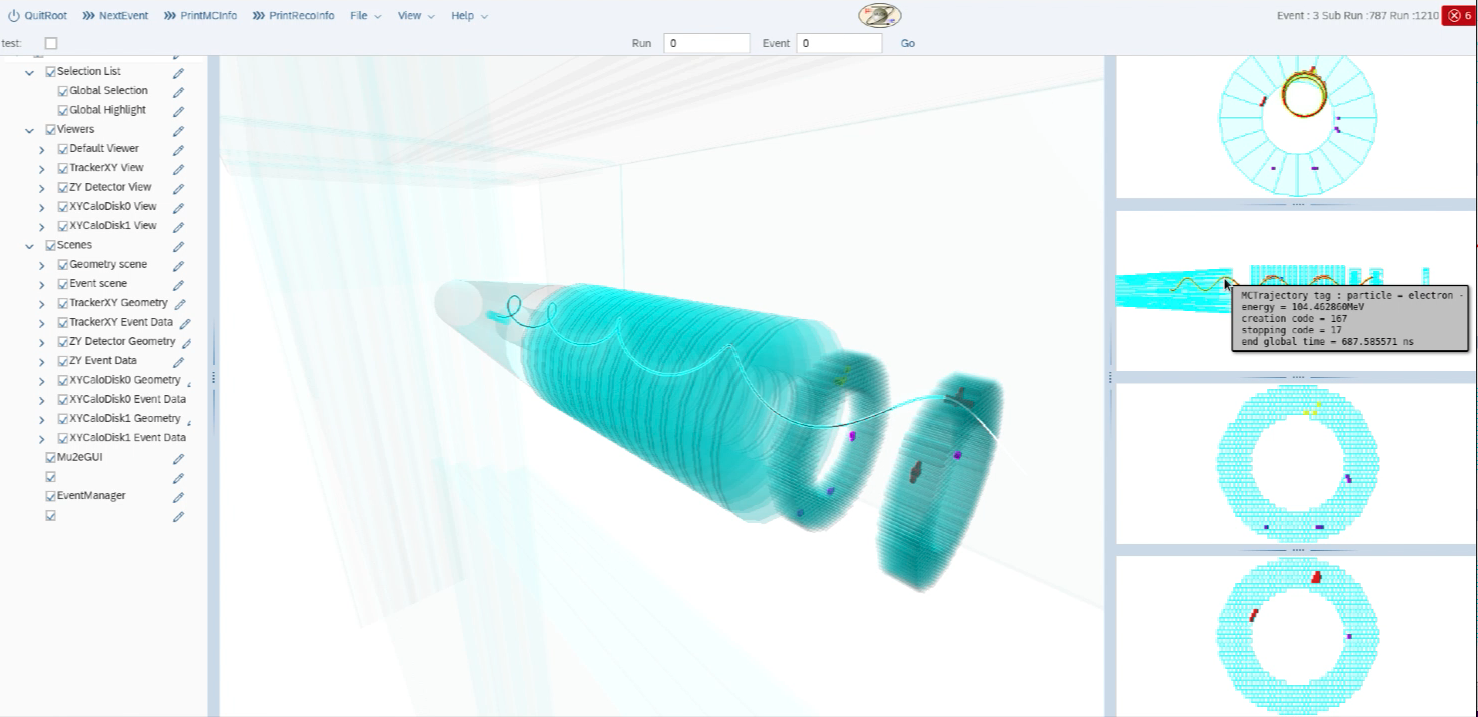
\includegraphics[width=0.9\linewidth]{figures/2D-REve-label.png}
\caption{\textbf{User Experience:} An example REveMu2e displaying a conversion entering the detector region and producing a helical track in the tracker and calorimeter. The MC truth trajectory is highlighted and a label is visible. The calorimeter cluster length is proportional to energy deposited, red indicates in is at a time close to the track time, the largest red cluster is clearlu a result of the conversion. The GUI is also visible along with the side panel of 2D views. To enlarge a 2D view the user simply selects from the "View" menu on the GUI. Two buttons at the top allow the user to "print" information to the terminal regarding the details of the event. The panel on the left allows users to remove event objects and geometries (to get a clearer view).}
\label{fig:teve_3D_label}
\end{center}
\end{figure}


 \begin{figure}[htb]
\begin{center}
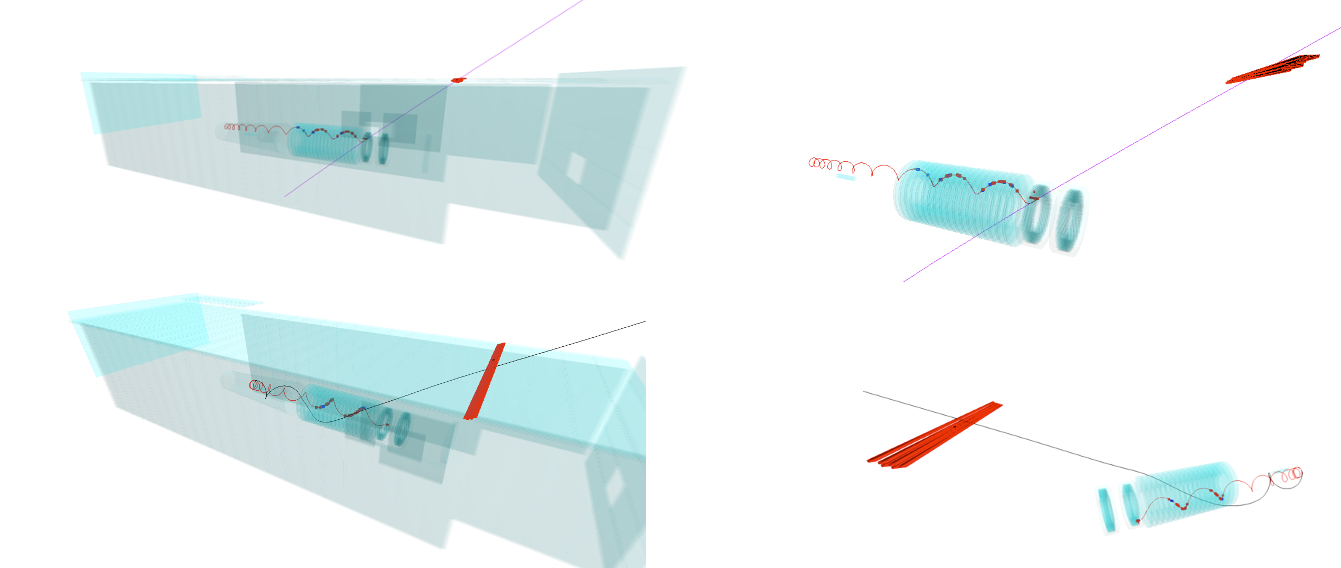
\includegraphics[width=0.9\linewidth]{figures/REve_cosmics.png}
\caption{\textbf{Example Cosmic Veto View:} An example REve displays of the showing a cosmic muon entering the detector region and producing the helical track in the tracker and calorimeter. The CRV bars that are hit are highlighted while the rest of the CRV remains light and translucent. The CRV can be removed easily using the GUI  (see plots on the right).}
\label{fig:teve_3D_cosmics}
\end{center}
\end{figure}




 \begin{figure}[htb]
\begin{center}
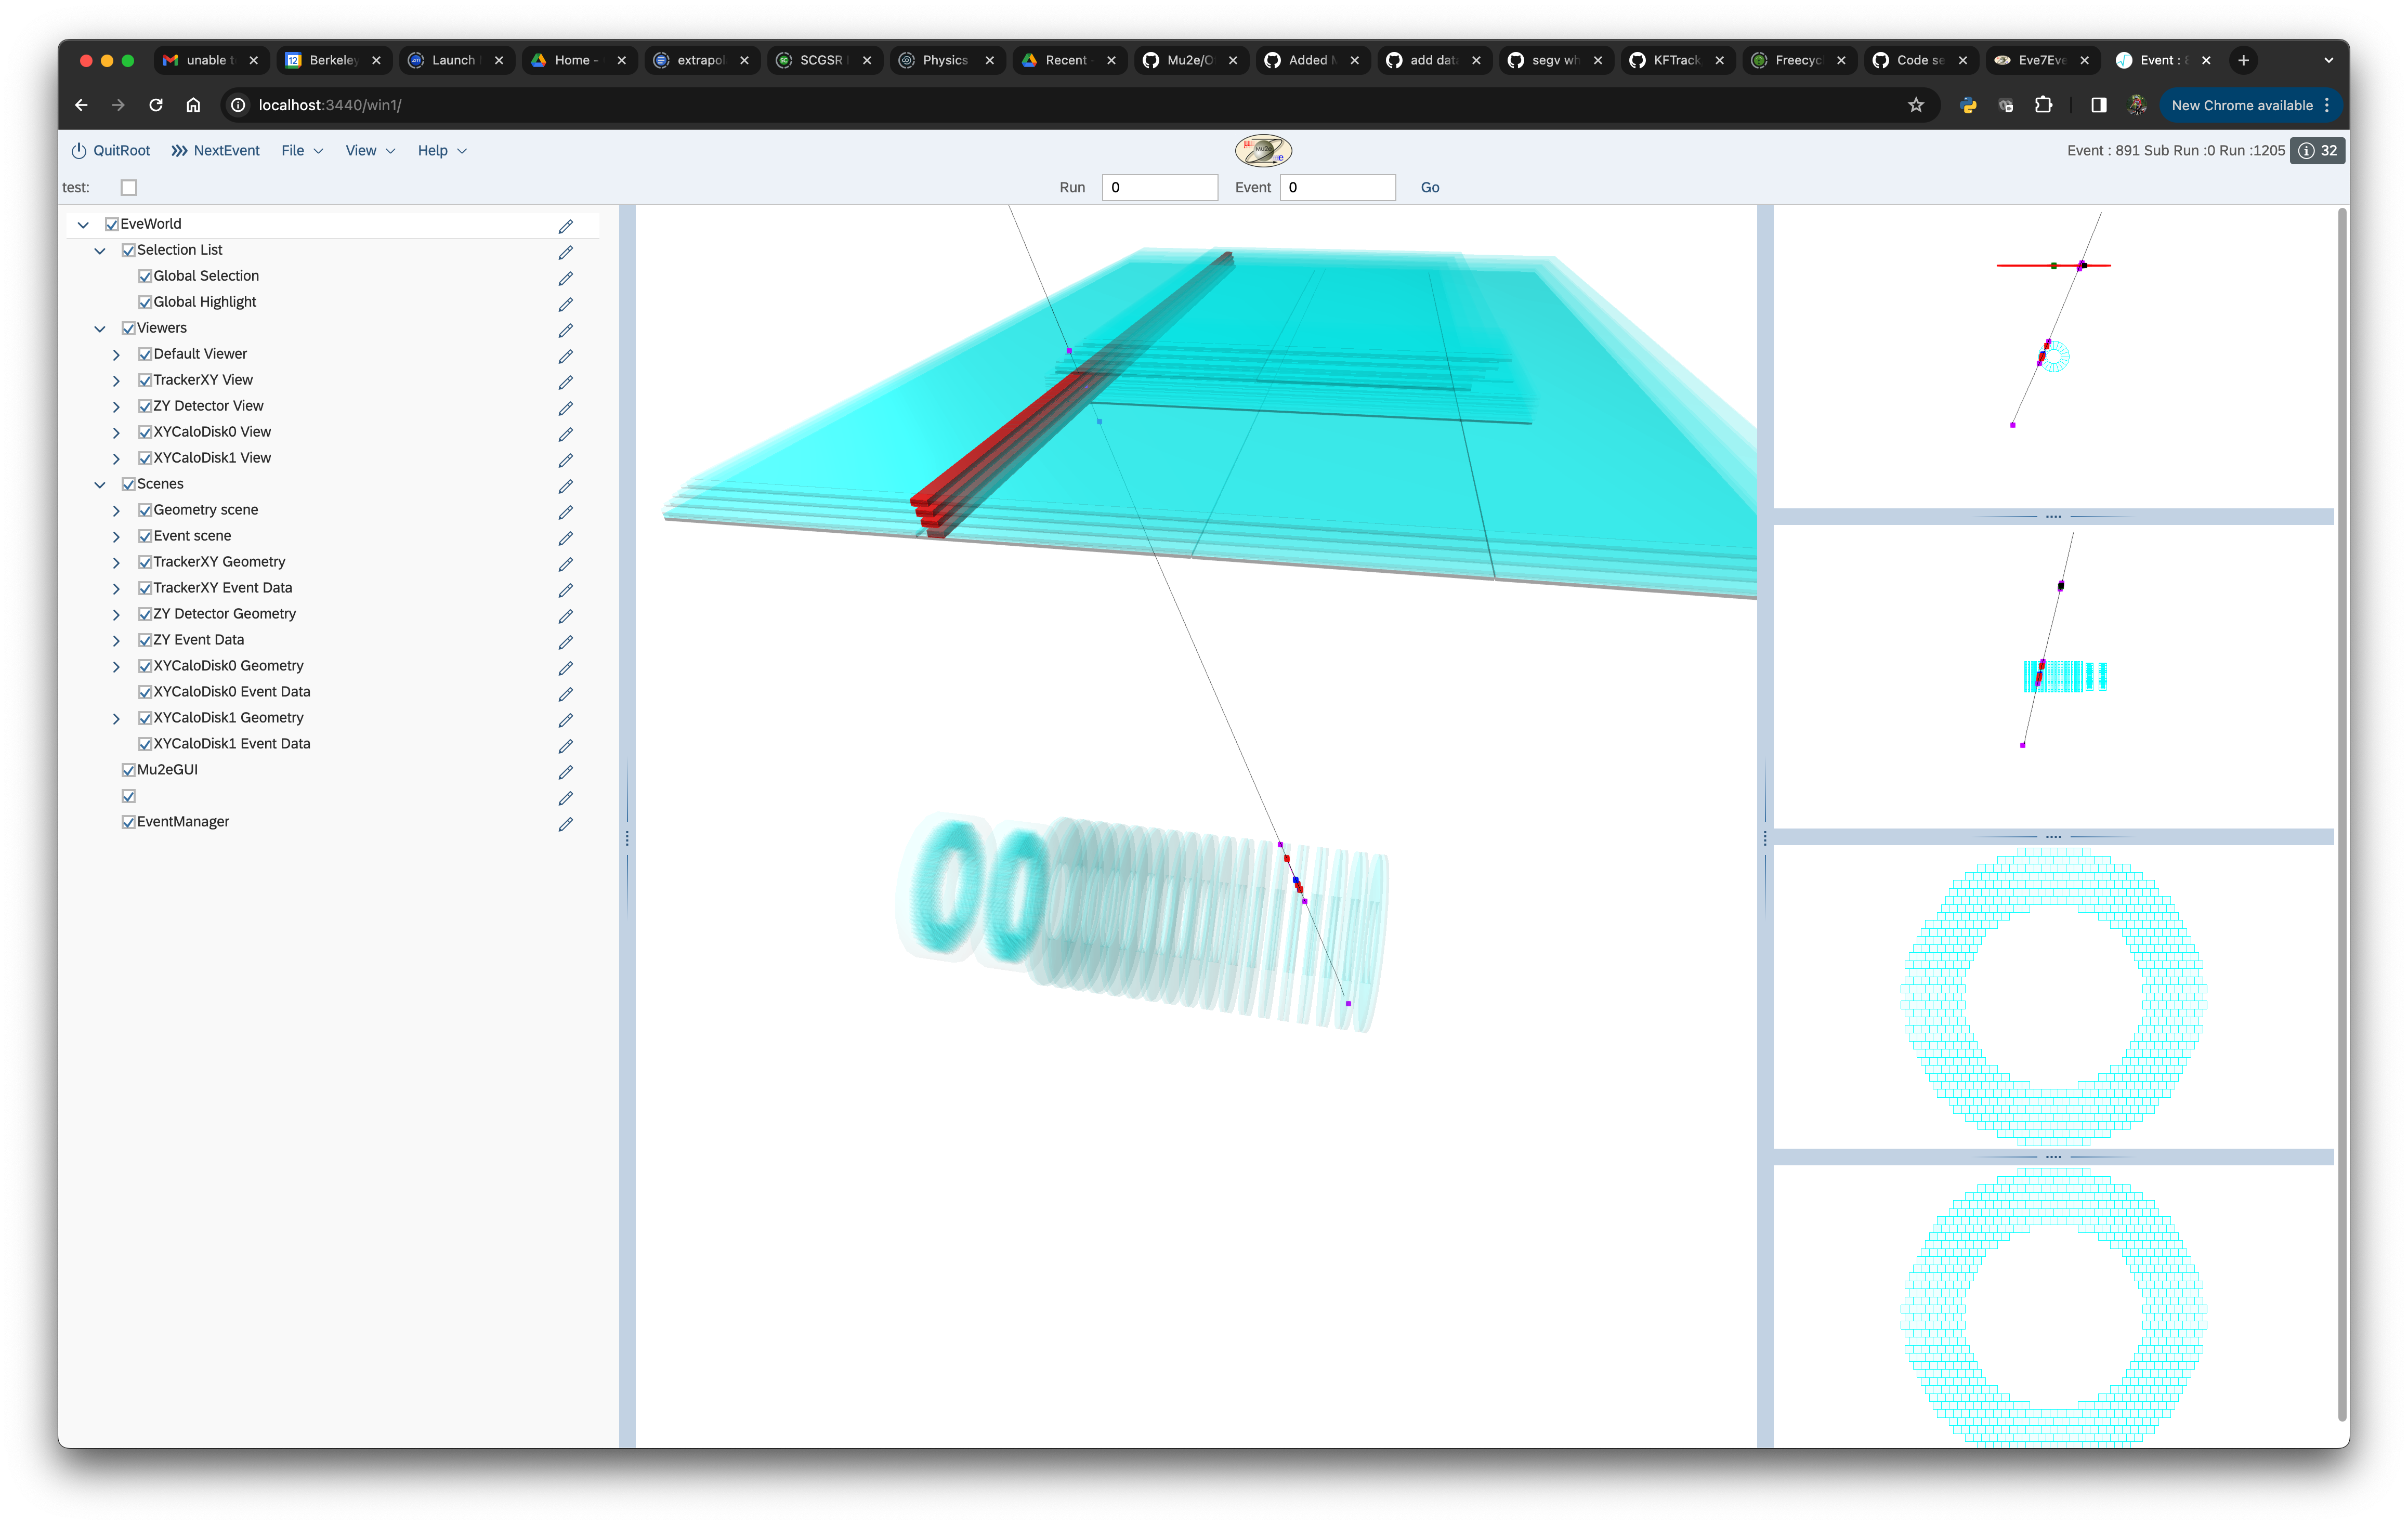
\includegraphics[width=0.9\linewidth]{figures/extracted.png}
\caption{\textbf{Extracted Cosmic View:}An example REve displays of the showing a cosmic muon entering the detector region in extracted (field off) configuration}
\label{fig:teve_3D_extracted}
\end{center}
\end{figure}

\subsubsection{REveMu2e: Two-Dimensional Displays}


Although 3D visualization is essential there are also several use cases for 2D visualization. In REveMu2e the user could select an XY and YZ view of the tracker along with XY views of each calorimeter disk (with crystal outlines). These are easy to navigate to using the "View" menu. Examples are shown in Figure~\ref{fig:teve_2d_all}. Additional views can be added easily if we see a need, but we assume any spatial possibility is easily accessible from a rotation of the 3D display.

We are looking into a useful way to present time information and this could be added as a plot (using an add-in of a TCanvas) or using REve objects.

 \begin{figure}[htb]
\begin{center}
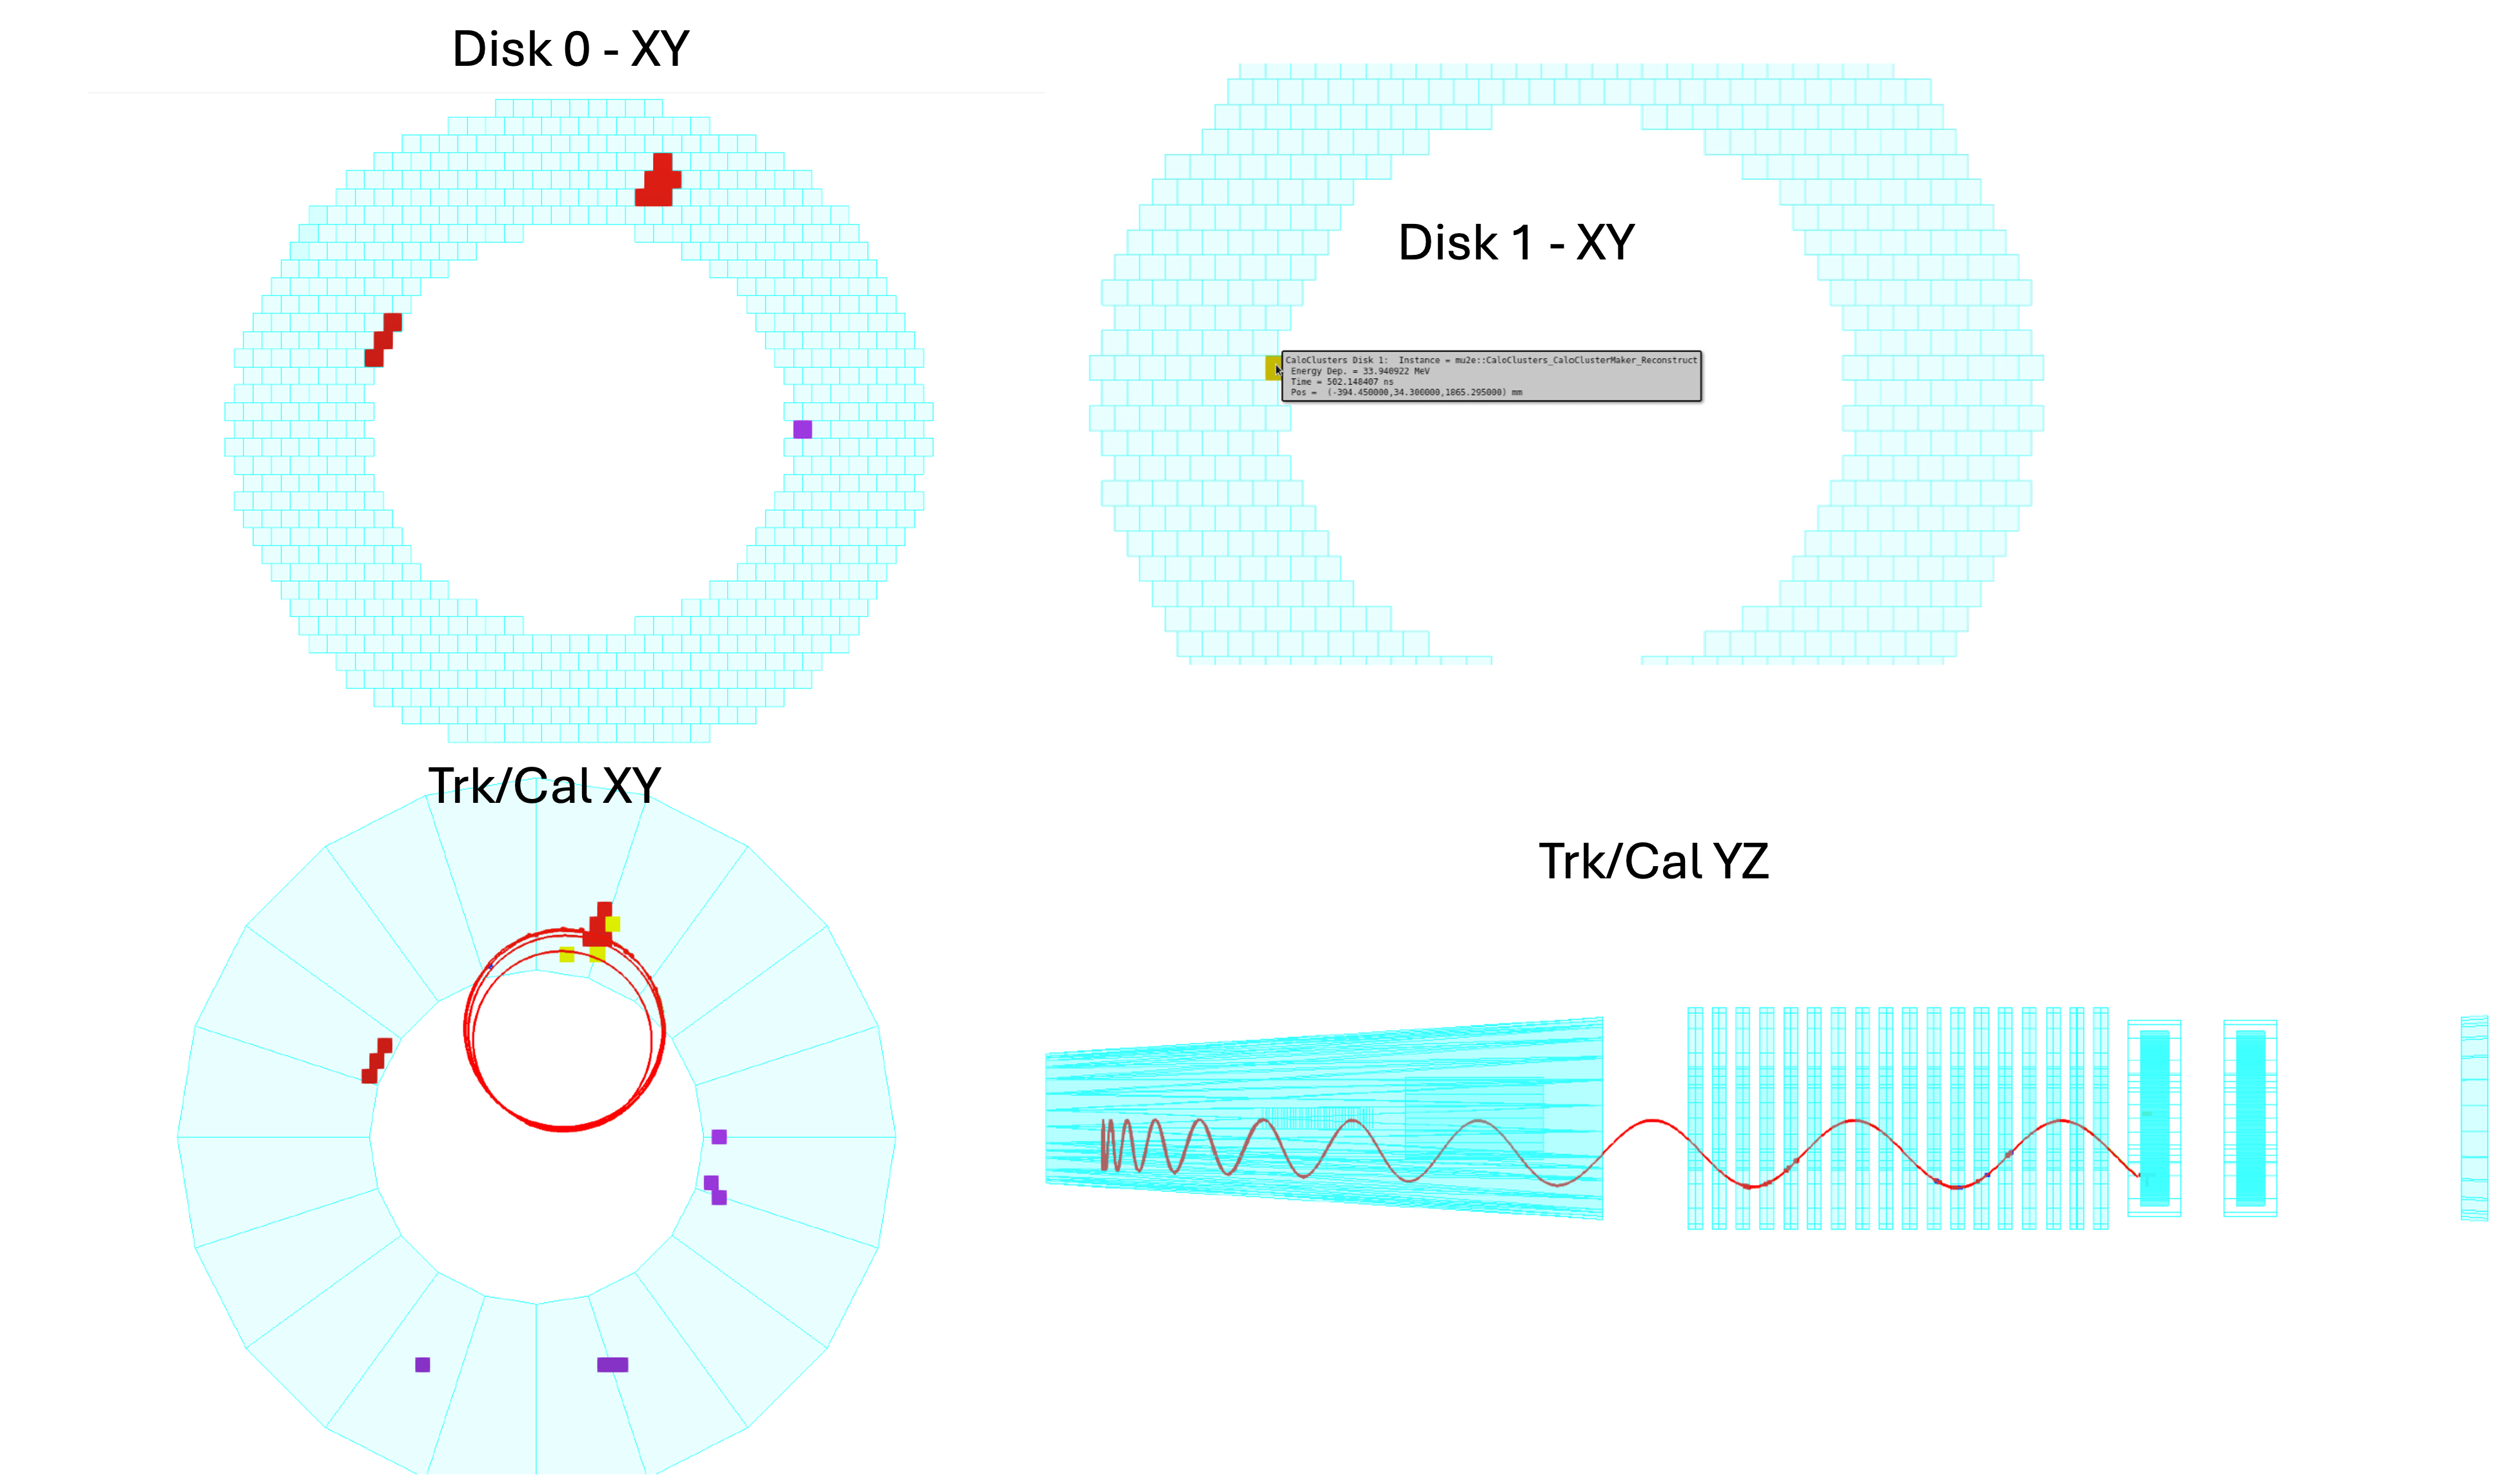
\includegraphics[width=0.9\linewidth]{figures/2D-REve-all.png}
\caption{\textbf{2D Examples: }An example displays in 2D for REveMu2e, showing both calorimeter disks and tracker views. Clusters are shown in larger squares and labeled. Crystal hits are shown in red. }
\label{fig:teve_2d_all}
\end{center}
\end{figure}



\section{Tutorials and Documentation (Sophie and Andy) }
\label{sec:tutorial}

%\textcolor{red}{Sophie: I added this. Do we want to mention this here? I feel this is a bigger topic than just our group so I made a new section. It might need to be somewhere else.}

\subsection{Documentation}

\subsubsection{wikis}

The Mu2e internal wiki acts as the main source of documentation on current software practices. 

\subsubsection{GitHub}

Developers of any of the official Mu2e packages must provide 
\subsection{Training Material}

In order to facilitate users we have developed detailed tutorials and documentation for the existing analysis tools.

\subsubsection{General Offline Computing Tutorials}

\subsubsection{TrkAna and REveMu2e}

Within the GitHub repositories for each of these packages are a set of basic tutorials that become more advanced as the user works through the examples.

In the case of TrkAna, tutorials for both python and ROOT C++-based analyses exist. The basic tutorial shows users how to import the information to their analysis platform, manipulate it, add selection cuts, and make basic histograms. The more advanced tutorials provide the user with a real analysis problem and show them how to perform maximum likelihood fits to a Mock Data sample to provide some estimate of the signal and background yields.

The REveMu2e tutorial starts by showing the user how to visualize tracks, hits and clusters in the three main detectors. It explains the interactive features and event navigation.

\subsubsection{Maintaining Material}
Training material is updated frequently as the software evolves. This allows users to always be able to run the tutorials out-of-the-box. Bi-annual in-person sessions are held, the frequency of these will increase as we on-board analyzers in the coming year.

\subsubsection{In-person Training Sessions}